\documentclass{cernyrep}
\begin{document}
\title{Particle ID performance of Liquid Argon TPC}
\author{J-PARC T32 collaboration}
\institute{(1) ETH Z\"urich, (2) Iwate, (3) KEK IPNS, (4) Waseda}
\maketitle

\begin{abstract}

We have collected 
J-PARC K1.1Br beamline

This paper describes a study of particle identification performance of
liquid Argon TPC (LArTPC) detector using well-defined charged particles
(pions, kaons, and protons) with momentum of ~800 MeV/$c$
obtained at J-PARC K1.1Br beamline.

We have build a LArTPC detector with fiducial mass of ~150 kg,
and injected the beam particle

\end{abstract}

%%%%%%%%%%%%%%%%%%%%%%%%%%%%%%%%%%%%%%%%%%%%%%%%%%
\section{Introduction}
%%%%%%%%%%%%%%%%%%%%%%%%%%%%%%%%%%%%%%%%%%%%%%%%%%
Refer \cite{Araoka:2011pw} for hardware/beam line description

%%%%%%%%%%%%%%%%%%%%%%%%%%%%%%%%%%%%%%%%%%%%%%%%%%
\section{Data Quality}
%%%%%%%%%%%%%%%%%%%%%%%%%%%%%%%%%%%%%%%%%%%%%%%%%%
\subsection{Collected Data}

Table~\ref{Table:Data} shows list of the collected data while Oct/2010 Run.
800 MeV/$c$ pion is expected to pass-through the detector as MIP,
and have uniform energy deposition to all the TPC channels.
So this data set is very useful for calibrating the detector response (See section xxx).
800 MeV/$c$ proton stops after ~15 cm of flight distance inside the TPC fiducial volume
with relatively large $dE/dx$. So we use the proton data set for validation of the
detector response at high $dE/dx$ region(See section xxx).
We have collected three different Kaon data by varying thickness of the degrader. 
540, 630, 680 MeV/$c$ are corresponds to the momentum degraded by 
2 lead glass, 1 lead glass + 1 lead block, and 1 lead glass, respectively, 
and such Kaon stops after 10 cm, 50 cm, and 65 cm of flight distance inside TPC fiducial volume.

Figure~\ref{Fig:Textbook} shows an 2D display of typical event 
taken with 800 MeV/$c$ electron trigger.
Horizontal axis corresponds to TPC channel number 
and zero means most upper stream strip. 
Since strip pitch is 1 cm, this is equivalent to
distance from beam injection point in cm.
Vertical axis corresponds to electron drift time in $\mu$s
and t=0 means trigger timing. In this TPC, anode and cathode is
located at top and bottom of the detector, respectively,
t=0 means energy deposition at anode and longer drift time 
means energy deposition in lower height.
With 200 V/cm of electric field, drift velocity is about 0.8 m/ms.
So drift of full detector (40 cm) takes 500 $\mu$s.
Color strength of the plot corresponds to the TPC signal pulse height
in ADC counts which is roughly proportional to $dE/dx$ of the track.
In this event, triggered electron can be clearly seen center of the detector
as an electromagnetic shower while there are two other particles 
accidentally overlapped with the triggered electron. 
Track at t=100 $\mu$s is considered as
a proton which stops after 15 cm of flight distance and 
has large $dE/dx$ around the stopped point.
Track at t=400 $\mu$s is considered as
a pion which passes-through the detector and 
has uniform $dE/dx$ over the TPC channels.
This event already gives us some idea for how good 
the particle identification performance of the LArTPC is.

Figure~\ref{Fig:Kmunu} shows a typical $K \to\mu\nu$ like event.
We can clearly identify a kink of the track at 60 cm which is considered
as stopped point of Kaon and it decays to  

Energy deposition of the track is about MIP at the injection point
and gradually increase towards the stopped point at 60 cm.



\begin{table}[h]
\begin{center}
\caption{List of collected data}
\begin{tabular}{l|ll}
  Particle  &Momentum (MeV/$c$) &Number of Events\\
\hline
  Pion      &800                &3,000\\
  Proton    &800                &1,500\\
  Kaon      &540 (2LG)          &7,000\\
  Kaon      &630 (1LG+1LB)      &40,000\\
  Kaon      &680 (1LB)          &35,000\\
  electron  &800                &2,500\\
  electron  &200                &10,000\\
  pion      &200                &10,000\\
\end{tabular}
\label{Table:Data}
\end{center}
\end{table}

\subsection{Beam Quality (Purity)}
\begin{itemize}
\item Plot: TREK counters (FC, GC, TOF) (A. Okamoto)
\item Plot: TOF before and after selection  (A. Okamoto)
\end{itemize}

 As described in section xx, we have several beam counters
to identify beam particles event by event
Figure~ref{fig:TREK} shows response of the, FC, GC, and TOF counters.
By using these counter information,

\begin{table}[h]
\begin{tabular}{llll}
  Particle  &FC(K) &FC(pi) &GC\\
  Pion      &x     &o      &x\\
  Kaon      &o     &x      &x\\
  Proton    &o     &x      &x\\
  electron  &x     &o      &o\\

\end{tabular}
\caption{List of collected data}
\label{Table:Data}
\end{table}


GC is used to identify electrons



 

\subsection{Beam Energy, Position}
\begin{itemize}
\item Plot: Proton momentum from TOF  (A. Okamoto)
\item Kaon:: Ongoing  (H. Okamoto?)
\item Plot: Beam position measurement
\end{itemize}

%%%%%%%%%%%%%%%%%%%%%%%%%%%%%%%%%%%%%%%%%%%%%%%%%%
\section{Software Framework}
%%%%%%%%%%%%%%%%%%%%%%%%%%%%%%%%%%%%%%%%%%%%%%%%%%

%%%%%%%%%%%%%%%%%%%%%%%%%%%%%%%%%%%%%%%%%%%%%%%%%%
\section{Event Reconstruction}
%%%%%%%%%%%%%%%%%%%%%%%%%%%%%%%%%%%%%%%%%%%%%%%%%%
\subsection{Noise Reduction}

Figure \ref{Fig:beforeFFT} shows raw waveform of the TPC signal
before applying any noise reduction. Two waveforms shown in this plot
are channel 13 and 37 in Figure~\ref{Fig:Textbook} which are roughly
proton stopped point and electron shower maximum point, respectively.
Signal-to-noise ratio for this particular case is poor and pion signal 
which is supposed to be t=400 $\mu$s is almost hidden by the noise. 
While time width of TPC signal is few $\mu$s which is determined by
drift time between anode and anode-grid, dominant noise component looks
higher frequency. To reduce such noises, we have applied FFT 
(Fast Flourier Transformation) filter to cut the high frequency component.
Figure \ref{Fig:FFT} shows amplitude as a function of frequency
for the same event. This clearly shows dominant noise component with
$>$ 200 kHz has good separation with signal component ($<$ 100 kHz).
Figure \ref{Fig:afterFFT} shows the waveform after removing high frequency
($>$ 80 kHz) component by the FFT filter. Signal-to-noise ratio is dramatically
improved. On the other hand, we expect certain bias to the signal charge
measurement by this filter, and it will be discussed in Section x.

\subsection{Hit Finding/Clustering}
\begin{itemize}
\item Plot: Finding efficiency vs threshold (Naganoma)
\item Plot: Through-going pion data Q vs pion (Tanaka)
\end{itemize}



\subsection{Stopped Point Finding}
\subsubsection{Proton}
\subsubsection{Kaon: Hough}
\subsubsection{Kaon: Chi2, BS}
\begin{itemize}
\item Plot: Proton Stopped point (A. Okamoto)
\item Plot: Hough Stopped point (Tanaka)
\item Plot: Chi2  Stopped point (H. Okamoto)
\item Plot: BS Stopped point (H. Okamoto)
\end{itemize}

%%%%%%%%%%%%%%%%%%%%%%%%%%%%%%%%%%%%%%%%%%%%%%%%%%
\section{Liquid Argon Purity}
%%%%%%%%%%%%%%%%%%%%%%%%%%%%%%%%%%%%%%%%%%%%%%%%%%


Attenuation of the drift electron depends on purity of liquid Argon.
So we need to apply correction to TPC signal charge depends on the drift time.
We use cosmic ray sample for measuring the liquid Argon purity,
and use this to correct the beam data.

Figure~{fig:CosmicEvent} shows an event display of typical cosmic muon event.
Figure~{fig:CosmicPurity} shows an drift electron lifetime as a function of
duration after initial filling.
Drift electron lifetime was 600 $\mu$s at 60 hours, and 400 $\mu$s after 150 hours.
Initial purity looks good, but the purity was slowly degrading
while data taking period.



\begin{itemize}
\item Plot: Typical Cosmic event (Naganoma)
\item Plot: Typical Lifetime Fit  (Naganoma)
\item Plot: Lifetime vs Time  (Naganoma)
\end{itemize}

%%%%%%%%%%%%%%%%%%%%%%%%%%%%%%%%%%%%%%%%%%%%%%%%%%
\section{Detector Simulation}
%%%%%%%%%%%%%%%%%%%%%%%%%%%%%%%%%%%%%%%%%%%%%%%%%%
\subsection{Geant3, recombination, drift velocity}

We use GEANT3 for simulating energy deposition of beam particles and
their daughters. Readout pitch is 1 cm, 

we set the maximum step of Geant to 0.5 mm
which is enough smaller than the readout pitch of 1 cm.

It means charge deposition in one strip is typically 
simulated with 20 GEANT steps.

We set energy cut-off for soft electron/photon emission to
10 keV which is minimum possible energy can be set in GEANT3.
This cut-off is very important for  ionization electron recombination.

Recombination of electron and Argon ion depends on
the electric field and $dE/dx$. We use a measurement in Ref.\cite{658352}.
\begin{equation}
Q = A \frac{Q_0}{1 + k dE/dx}, A = 0.800, k = 0.486
\end{equation}

Velocity of the drift electron depends on the liquid Argon temperature
and the electric field. We use a measurement in Ref \cite{649233}.


\begin{verbatim}
 *     Special TPAR for TMED   3   Liquid_argon                                                    *
 *  CUTGAM= 10.00 keV  CUTELE= 10.00 keV  CUTNEU= 10.00 MeV  CUTHAD= 10.00 MeV  CUTMUO= 10.00 MeV  *
 *  BCUTE = 10.00 keV  BCUTM = 10.00 keV  DCUTE = 10.00 keV  DCUTM = 10.00 keV  PPCUTM= 10.00 MeV  *
 *  IPAIR=  1.  ICOMP=  1.  IPHOT=  1.  IPFIS=  0.  IDRAY=  1.  IANNI=  1.  IBREM=  1.  IHADR=  4. *
 *  IMUNU=  1.  IDCAY=  1.  ILOSS=  1.  IMULS=  1.  IRAYL=  0.  ILABS=  0.  ISYNC=  0.  ISTRA=  0. *
\end{verbatim}



\begin{itemize}
\item Plot: Geant Geometry, typical track (Tanaka)
\item Plot: recombination factor, drift velocity  (Tanaka)
\end{itemize}

\subsection{Electric Field}

Electric field of the TPC field cage
We have calculated the electric field using a 2D FEM (Finite Element Method) package \cite{Ref:FEMTET}.

This field map is used for simulating electron drift.


\begin{itemize}
\item Plot: 2D field map  (Tanaka)
\end{itemize}

\subsection{Drift Electron Diffusion}
\begin{itemize}
\item Plot: drift simulation  (Tanaka)
\end{itemize}

\subsection{Preamp Gain Calibration}
\begin{itemize}
\item Preamp gain vs channel number  (Naito)
\end{itemize}

\subsection{FFT Noise}
\begin{itemize}
\item Plot: simulated event  (Nagasaka)
\end{itemize}

\subsection{Cross Talk}
\begin{itemize}
\item Plot: signal waveform (proton stopped point + 1)  (A. Okamoto)
\item Plot: simulated event with and without cross talk (A. Okamoto)
\end{itemize}

\subsection{Signal and Noise Scale Tuning}
\begin{itemize}
\item Plot: Landau distribution after the tuning  (Tanaka)
\end{itemize}

%%%%%%%%%%%%%%%%%%%%%%%%%%%%%%%%%%%%%%%%%%%%%%%%%%
\section{Data- MC Comparison}
%%%%%%%%%%%%%%%%%%%%%%%%%%%%%%%%%%%%%%%%%%%%%%%%%%
\subsection{Through-going Pion}
\begin{itemize}
\item Plot: Data-MC comparison  (Tanaka)
\end{itemize}

\subsection{Stopped Proton}
\begin{itemize}
\item Plot: Hit charge, cluster charge, stopped point  (A. Okamoto)
\item Plot: hit charge with different distance from SP   (A. Okamoto)
\item Plot: average hit charge vs different distance from SP   (A. Okamoto)
\end{itemize}

\subsection{Stopped Kaon}
\begin{itemize}
\item Plot: Hit charge, cluster charge, stopped point   (H. Okamoto)
\item Plot: hit charge with different distance from SP    (H. Okamoto)
\item Plot: average hit charge vs different distance from SP    (H. Okamoto)
\end{itemize}

%%%%%%%%%%%%%%%%%%%%%%%%%%%%%%%%%%%%%%%%%%%%%%%%%%
\section{Summary}
%%%%%%%%%%%%%%%%%%%%%%%%%%%%%%%%%%%%%%%%%%%%%%%%%%
\clearpage

\begin{figure}[htbp]
 \begin{center}
  \includegraphics[width=100mm]{Textbook.eps}
 \end{center}
 \caption{Event display of 800 MeV/$c$ electron triggered event.
Accidentally overlapped with a proton and a pion.}
 \label{Fig:Textbook}
\end{figure}

\begin{figure}[htbp]
 \begin{center}
  \includegraphics[width=100mm]{Kmunu.eps}
 \end{center}
 \caption{Event display of Kaon 630 MeV/$c$ triggered event}
 \label{Fig:Kmunu}
\end{figure}

\begin{figure}[htbp]
 \begin{center}
  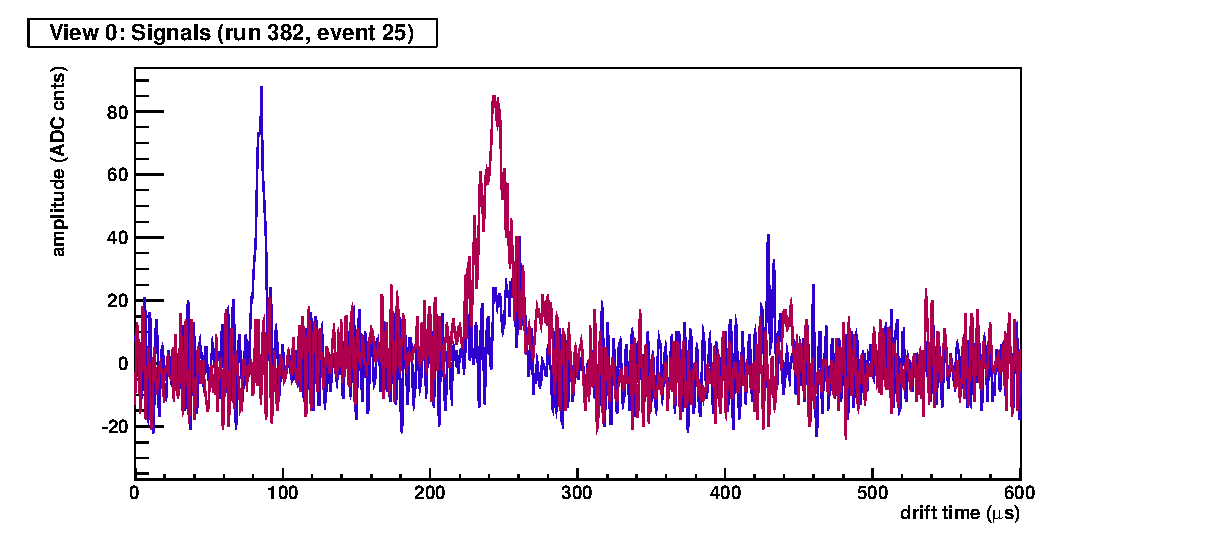
\includegraphics[width=100mm]{beforeFFT.eps}
 \end{center}
 \caption{TPC raw signal waveform for "Textbook" event channel 13 and 37.}
 \label{Fig:beforeFFT}
\end{figure}

\begin{figure}[htbp]
 \begin{center}
  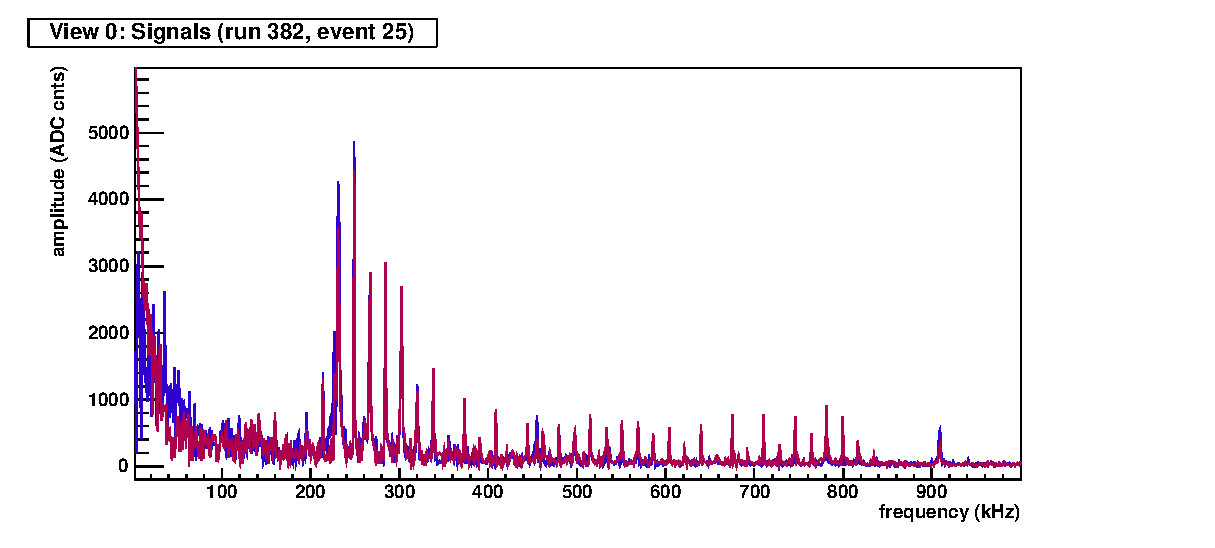
\includegraphics[width=100mm]{FFT.eps}
 \end{center}
 \caption{FFT frequency amplitude distribution}
 \label{Fig:beforeFFT}
\end{figure}

\begin{figure}[htbp]
 \begin{center}
  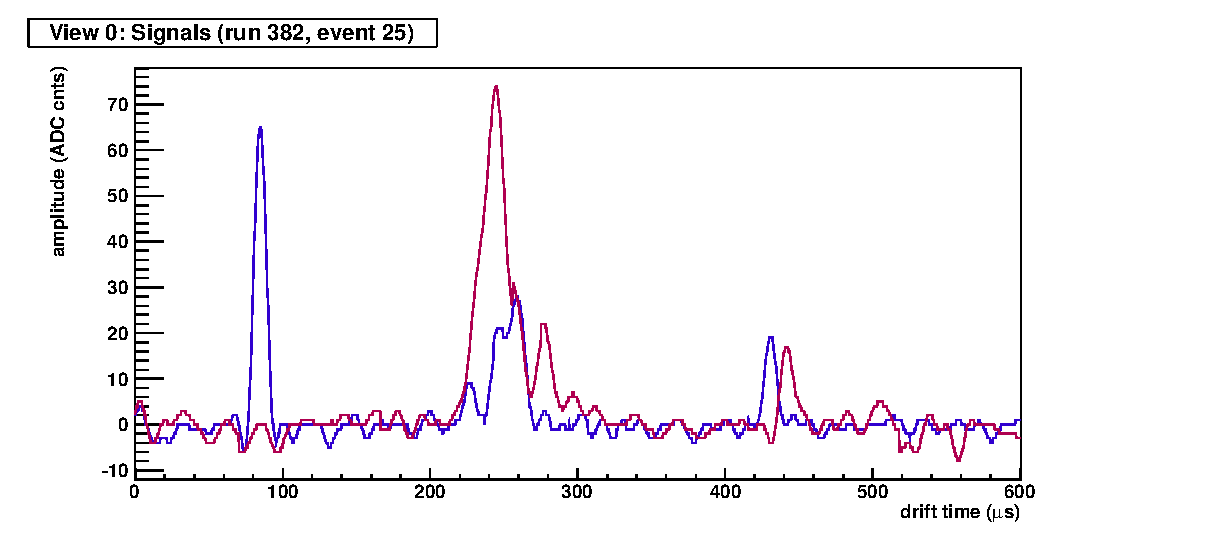
\includegraphics[width=100mm]{afterFFT.eps}
 \end{center}
 \caption{TPC signal waveform after cutting the frequency $>$ 80 kHz.}
 \label{Fig:afterFFT}
\end{figure}


\begin{figure}[htbp]
 \begin{center}
  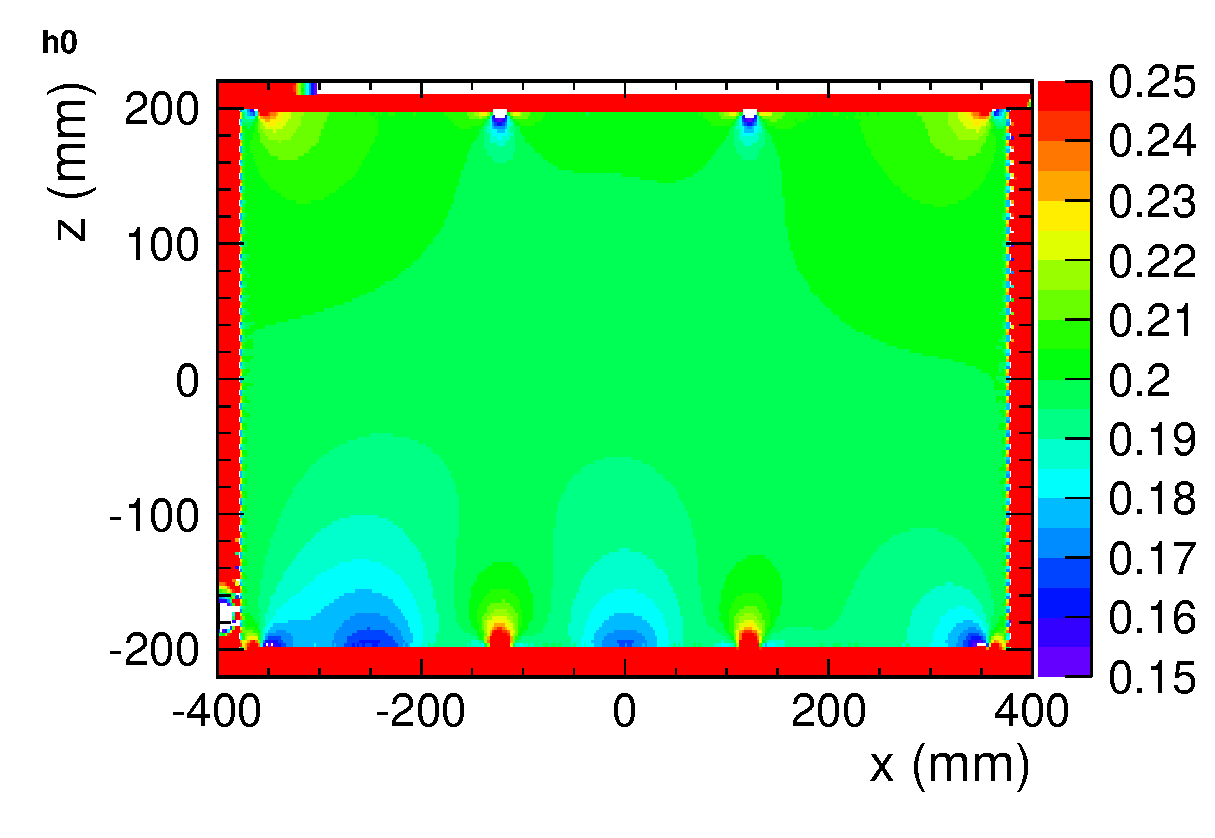
\includegraphics[width=100mm]{2DFieldMap.eps}
 \end{center}
 \caption{Electric field map obtained from 2D FEM calculation}
 \label{fig:2DFieldMap}
\end{figure}

\begin{figure}[htbp]
 \begin{center}
  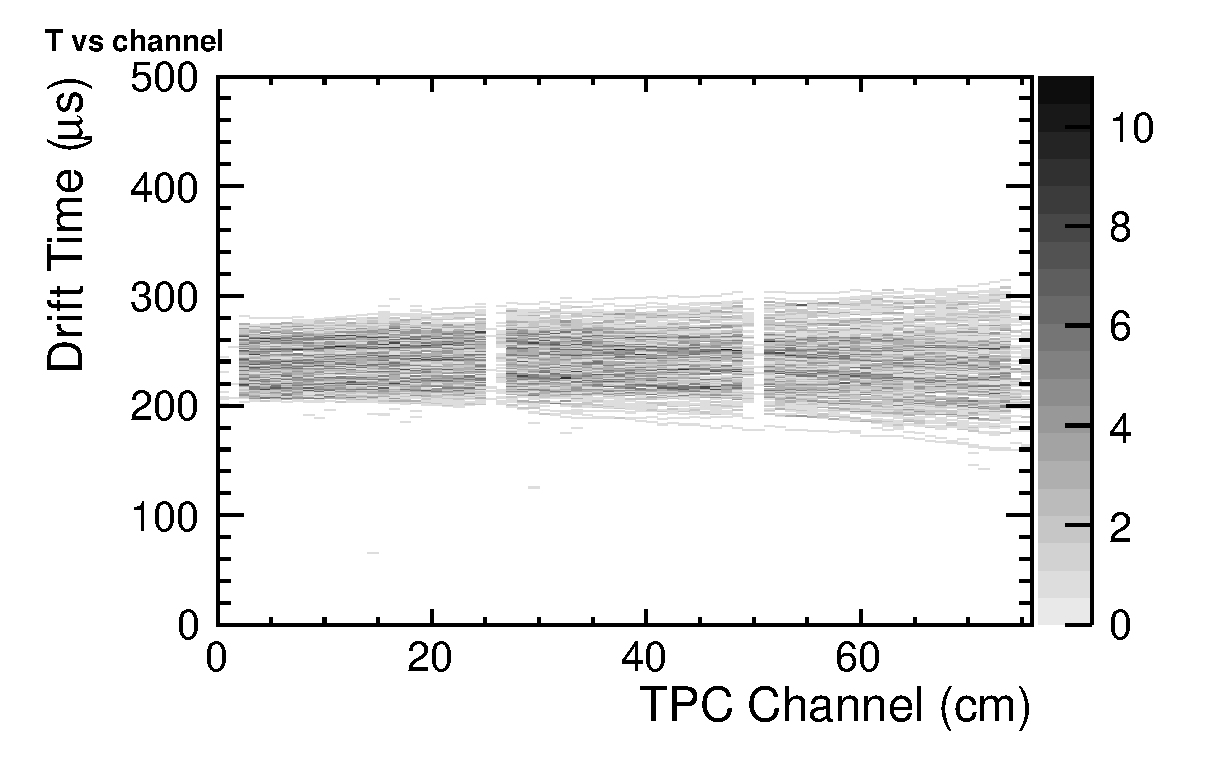
\includegraphics[width=100mm]{PionTrack.eps}
 \end{center}
 \caption{800 MeV/c pion sample}
 \label{fig:PionTrack}
\end{figure}

\begin{figure}[htbp]
 \begin{center}
  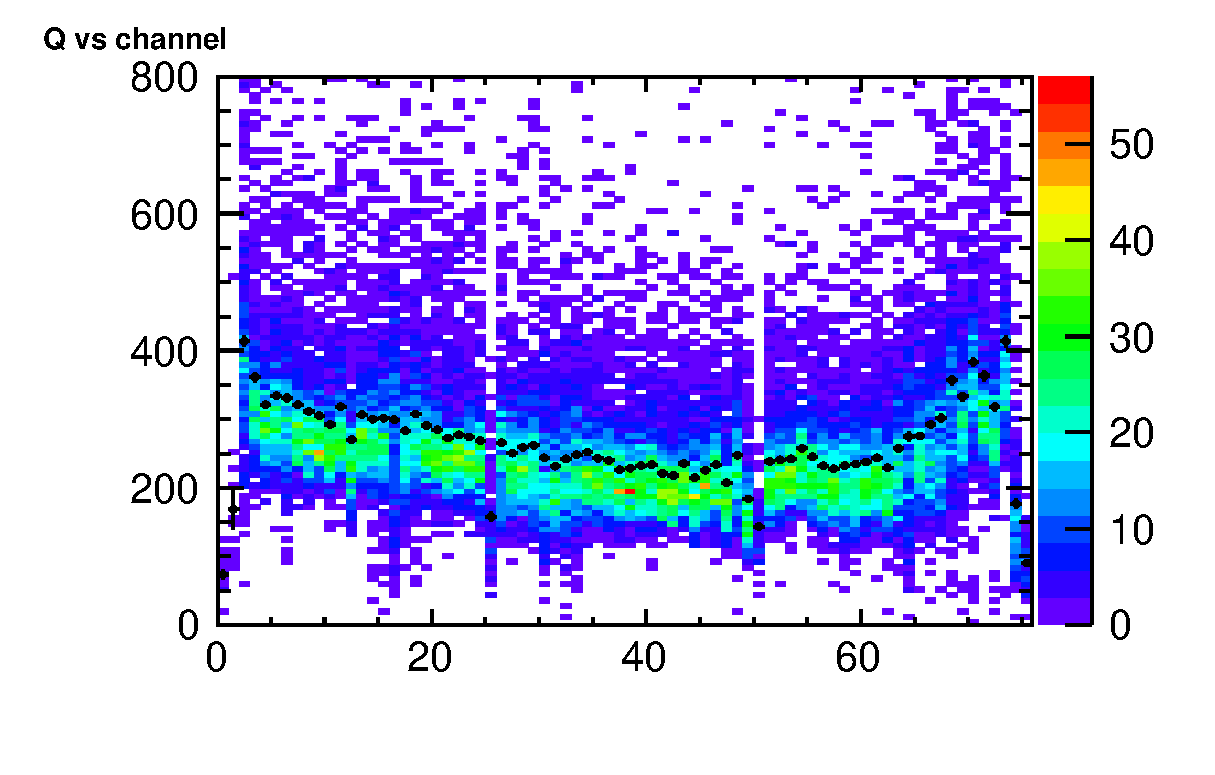
\includegraphics[width=100mm]{PionQvsCh.eps}
 \end{center}
 \caption{800 MeV/c pion average hit charge}
 \label{fig:PionQvsCh}
\end{figure}

\begin{figure}[htbp]
 \begin{center}
  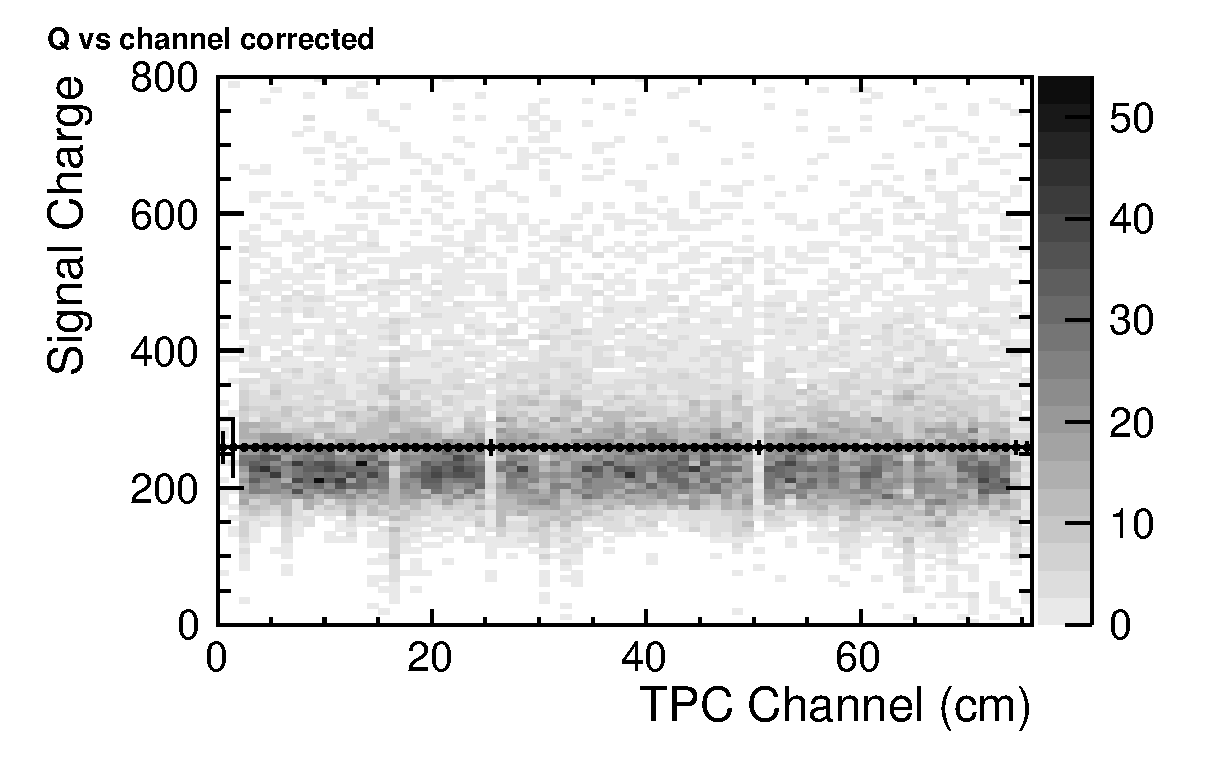
\includegraphics[width=100mm]{PionQcvsCh.eps}
 \end{center}
 \caption{800 MeV/c pion average hit charge after calibration}
 \label{fig:PionQcvsCh}
\end{figure}

\begin{figure}[htbp]
 \begin{center}
  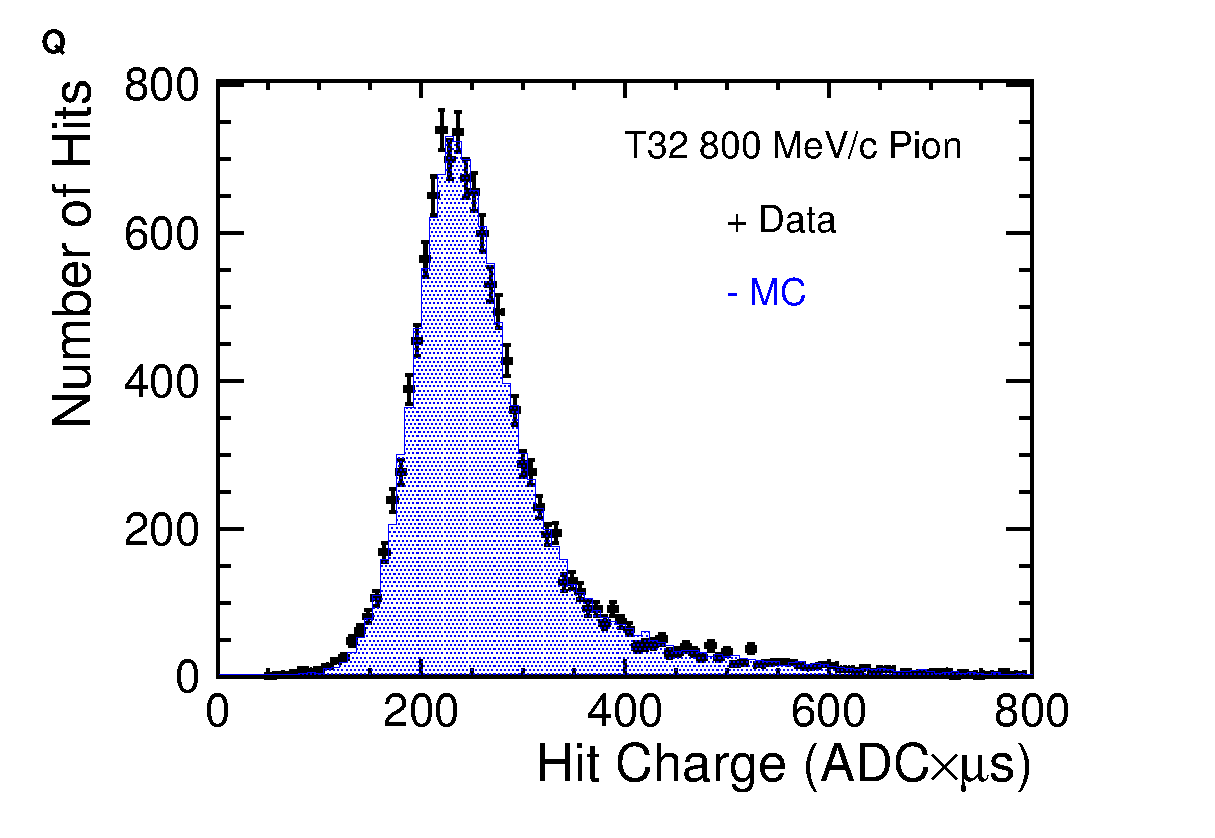
\includegraphics[width=100mm]{PionLandau.eps}
 \end{center}
 \caption{800 MeV/c pion Landau distribution}
 \label{fig:PionLandau}
\end{figure}

\begin{figure}[htbp]
 \begin{center}
  \includegraphics[width=100mm,bb=0 0 861 556]{KaonDataMC.png}
 \end{center}
 \caption{Data-MC comparison for several Kaon quantities}
 \label{fig:KaonDataMC}
\end{figure}

\begin{figure}[htbp]
 \begin{center}
  \includegraphics[width=100mm,bb=0 0 861 556]{KaonQvsR.png}
 \end{center}
 \caption{Kaon hit charge distribution for different distance from the stopped point.}
 \label{fig:KaonQvsR}
\end{figure}

\begin{figure}[htbp]
 \begin{center}
  \includegraphics[width=100mm,bb=0 0 861 556]{KaonQvsR2.png}
 \end{center}
 \caption{Kaon average hit charge as a function of distance from the stopped point.}
 \label{fig:KaonQvsR2}
\end{figure}

\begin{figure}[htbp]
 \begin{center}
  \includegraphics[width=100mm,bb=0 0 861 566]{KaonQRvsR.png}
 \end{center}
 \caption{Data/MC ratio of the proton average hit charge as a function of distance from the stopped point.}
 \label{fig:KaonQRvsR}
\end{figure}

\begin{figure}[htbp]
 \begin{center}
  \includegraphics[width=100mm,bb=0 0 1196 973]{ProtonQvsR.png}
 \end{center}
 \caption{Proton hit charge distribution for different distance from the stopped point.}
 \label{fig:ProtonQvsR}
\end{figure}

\begin{figure}[htbp]
 \begin{center}
  \includegraphics[width=100mm,bb=0 0 393 376]{ProtonQvsR2.png}
 \end{center}
 \caption{Proton average hit charge as a function of distance from the stopped point.}
 \label{fig:ProtonQvsR2}
\end{figure}

\begin{figure}[htbp]
 \begin{center}
  \includegraphics[width=50mm,bb=0 0 426 413]{ProtonQRvsR.png}
 \end{center}
 \caption{Data/MC ratio of the proton average hit charge as a function of distance from the stopped point.}
 \label{fig:ProtonQRvsR}
\end{figure}


\clearpage

\begin{thebibliography}{99}
%\cite{Araoka:2011pw}
\bibitem{Araoka:2011pw}
  O.~Araoka {\it et al.},
  %``A tagged low-momentum kaon test-beam exposure with a 250L LAr TPC (J-PARC
  %T32),''
  J.\ Phys.\ Conf.\ Ser.\  {\bf 308}, 012008 (2011)
  [arXiv:1105.5818 [physics.ins-det]].
  %%CITATION = 00462,308,012008;%%

\bibitem{Mihara:2004ft}
S.~Mihara [MEG Collaboration],
%``R&D work on a liquid-xenon photon detector for MEG experiment at PSI,''
Nucl.\ Instrum.\ Meth.\ A {\bf 518}, 45 (2004).
%%CITATION = NUIMA,A518,45;%%

%\cite{658352}
\bibitem{658352} 
  S.~Amoruso {\it et al.} [ICARUS Collaboration],
  %``Study of electron recombination in liquid argon with the ICARUS TPC,''
  Nucl.\ Instrum.\ Meth.\ A\ {\bf 523}, 275  (2004).
  %%CITATION = NUIMA,A523,275;%%

%\cite{649233}
\bibitem{649233} 
  S.~Amoruso, M.~Antonello, P.~Aprili, F.~Arneodo, A.~Badertscher, B.~Baibusinov, M.~Baldo-Ceolin and G.~Battistoni {\it et al.},
  %``Analysis of the liquid argon purity in the ICARUS T600 TPC,''
  Nucl.\ Instrum.\ Meth.\ A\ {\bf 516}, 68  (2004).
  %%CITATION = NUIMA,A516,68;%%
\end{thebibliography}


\end{document}
